%%%%%%%%%%%%%%%%%%%%%%%%%%%%%%%%%%%%%%%%%%%%%%%%%%%%%%%%%%
%
% Vzor pro sazbu kvalifikační práce
%
% Západočeská univerzita v Plzni
% Fakulta aplikovaných věd
% Katedra informatiky a výpočetní techniky
%
% Petr Lobaz, lobaz@kiv.zcu.cz, 2016/03/14
%
%%%%%%%%%%%%%%%%%%%%%%%%%%%%%%%%%%%%%%%%%%%%%%%%%%%%%%%%%%

% Možné jazyky práce: czech, english
% Možné typy práce: BP (bakalářská), DP (diplomová)
\documentclass[czech,DP]{thesiskiv}

% Definujte údaje pro vstupní strany
%
% Jméno a příjmení; kvůli textu prohlášení určete, 
% zda jde o mužské, nebo ženské jméno.
\author{Bc. František Koleňák}
\declarationmale

%alternativa: 
%\declarationfemale

% Název práce
\title{Klasifikace chyb SW \\na základě analýz z úložiště}

% 
% Texty abstraktů (anglicky, česky)
%
\abstracttexten{The text of the abstract (in English). It contains the English translation of the thesis title and a short description of the thesis.}

\abstracttextcz{Text abstraktu (česky). Obsahuje krátkou anotaci (cca 10 řádek) v češtině. Budete ji potřebovat i při vyplňování údajů o bakalářské práci ve STAGu. Český i anglický abstrakt by měly být na stejné stránce a měly by si obsahem co možná nejvíce odpovídat (samozřejmě není možný doslovný překlad!).
}

% Na titulní stranu a do textu prohlášení se automaticky vkládá 
% aktuální rok, resp. datum. Můžete je změnit:
%\titlepageyear{2016}
%\declarationdate{1. března 2016}

% Ve zvláštních případech je možné ovlivnit i ostatní texty:
%
%\university{Západočeská univerzita v Plzni}
%\faculty{Fakulta aplikovaných věd}
%\department{Katedra informatiky a výpočetní techniky}
%\subject{Bakalářská práce}
%\titlepagetown{Plzeň}
%\declarationtown{Plzni}

%%%%%%%%%%%%%%%%%%%%%%%%%%%%%%%%%%%%%%%%%%%%%%%%%%%%%%%%%%
%
% DODATEČNÉ BALÍČKY PRO SAZBU
% Jejich užívání či neužívání záleží na libovůli autora 
% práce
%
%%%%%%%%%%%%%%%%%%%%%%%%%%%%%%%%%%%%%%%%%%%%%%%%%%%%%%%%%%

% Zařadit literaturu do obsahu
\usepackage[nottoc,notlot,notlof]{tocbibind}

% Umožňuje vkládání obrázků
\usepackage[pdftex]{graphicx}

% Odkazy v PDF jsou aktivní; navíc se automaticky vkládá
% balíček 'url', který umožňuje např. dělení slov
% uvnitř URL
\usepackage[pdftex]{hyperref}
\hypersetup{colorlinks=true,
  unicode=true,
  linkcolor=black,
  citecolor=black,
  urlcolor=black,
  bookmarksopen=true}

% Při používání citačního stylu csplainnatkiv
% (odvozen z csplainnat, http://repo.or.cz/w/csplainnat.git)
% lze snadno modifikovat vzhled citací v textu
\usepackage[numbers,sort&compress]{natbib}

%%%%%%%%%%%%%%%%%%%%%%%%%%%%%%%%%%%%%%%%%%%%%%%%%%%%%%%%%%
%
% VLASTNÍ TEXT PRÁCE
%
%%%%%%%%%%%%%%%%%%%%%%%%%%%%%%%%%%%%%%%%%%%%%%%%%%%%%%%%%%
\begin{document}
%
\maketitle

\addtocontents{toc}{\protect\thispagestyle{empty}}
\addtocontents{toc}{\protect\pagestyle{empty}}
\tableofcontents
\thispagestyle{empty}

\chapter{Úvod}
\setcounter{page}{1}
%V souboru \texttt{literatura.bib} jsou uvedeny příklady, jak citovat knihu \cite{KnuthAOCP2}, článek v časopisu \cite{Hoare1961}, webovou stránku \cite{Graphics2D}.
 
\newpage

\chapter{Řízení projektů}
Řízení projektu (někdy též projektové řízení) se zabývá řízením projektu, tedy časově ohraničené a ucelené sady činností a procesů, jejímž cílem je co nejefektivněji zavést, vytvořit nebo změnit něco konkrétního (definováno daným projektem).

Tradiční přístup řízení projektů je založen na důkladném naplánování na začátku projektu a řízení všech aktivit v průběhu projektu. Tento přístup (též známý jako vodopádový model) je nejvíce vhodný na projekty, které mají podobu cíle jasně danou a neměnnou (chodník, dům) a ve kterých je nutné dobře naplánovat všechny aktivity související s daným projektem. Tradiční přístup vyžaduje kvalitně popsaný cíl, výstupy a plán projektu.

Opakem tradičního přístupu je agilní přístup. Ten je založen na průběžném upřesňování cíle, díky interakci se zákazníkem či s uživateli výsledků projektu. Tento proces se označuje jako získávání zpětné vazby. Reagováním na vstupy od zákazníka je projekt dynamicky upravován a proto je vhodný na takové projekty, kde dochází k vývoji produktu, tedy tehdy když nelze předem kvalitně popsat a naplánovat vše do podrobností a bez zpětné vazby. Agilní přístup se často používá ve vývoji software.

\section{Fáze projektu}
Projekt se může nacházet v různých fázích (procesních skupinách). Tyto fáze se mohou lišit použitou metodou na řízení projektu, ale víceméně je struktura a podoba fází velice podobná. Nejčastějšími fázemi jsou:

\begin{itemize}
	\item {Zahájení} - Start projektu a vytyčení jeho mezí
	\item {Plánování} - Plánování částí projektu
	\item {Realizace} - Implementace rozplánované části
	\item {Monitorování a řízení} - Zpětná vazba od zákazníka, podpora
	\item {Uzavření} - Oficiální ukončení projektu
\end{itemize}

%TODO moznost pridat podrobnosti k jednotlivym fazim

\begin{figure}[!ht]
\begin{center}
	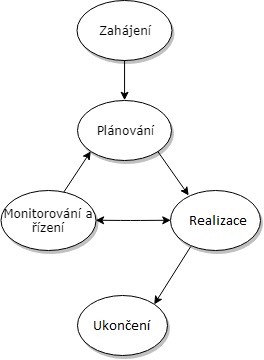
\includegraphics[scale=1.25]{Pic/planingDiagram.png}
\end{center}
\label{pic:planingDiagram}
\caption{Plánovací diagram}
\end{figure}


Projekt začíná zahájením a končí uzavřením. Fáze plánování, realizace a monitorování a řízení se mohou opakovat až do ukončení projektu. Diagram fází viz Obrázek \ref{pic:planingDiagram}. Vodopádový model má pak jednotlivé fáze za sebou tak, že přechod do další fáze je až tehdy, když je daná fáze kompletně ukončena.

\section{Softwarové chyby}
Softwarové chyba (také nazývána jako \uv{softwarový bug}) se dá definovat jako chyba, defekt, porucha či selhání v počítačovém programu nebo systému, která způsobuje vytváření nekorektních nebo neočekávaných výsledků a nebo nezamýšlené chování. 

Softwarové chyby, jsou nedílnou součástí každého softwaru. Projekt větších rozměrů bez žádné softwarové chyby je velmi vzácný, tedy se dá předpokládat, že v nějaké fázi vývoje se objeví nějaký bug. Proces hledání a řešení bugů je nazýván jako \uv{debugování} a často používá techniky nebo nástroje pro určení bugu. 

\subsection{Testování aplikací}
Testování aplikací slouží pro zamezení vydání produktu, který obsahuje chyby jakéhokoliv druhu. Testy mají vliv na kvalitu výsledného produktu, tím pádem se snaží pokrýt co nejvíce případů použití, které mohou nastat.

Samotné bugy vznikají již při realizaci daného projektu a jsou často nalezeny při testování daného řešení samotným vývojářem, nebo nástroji používanými pro překlad a vývoj. Takovýmto testů se říká \uv{Assembly tests}. Další proces, používaný pro nalezení bugů, je takzvaný \uv{code review}, tedy revize kódu. Při tomto procesu se na cizí kód(vytvořený jiným vývojářem) podívá další vývojář a překontroluje kód, za účelem ověření funkcionality a nalezení potencionálních problémů, které původního autora kódu nemusely napadnout. 

Dalším zdrojem odhalení bugů je automatizované testování kódu. Existuje spoustu druhů technik testování. Jedním z hojně používaných druhů testů jsou takzvané jednotkové testy. Ty z pravidla píší samotní vývojáři a slouží k ověření funkcionality části kódu, na co nejmenších úsecích kódu, zpravidla na jednotlivé třídy a metody. Hlavním účelem těchto testů je odhalení funkční chyby v případě, že je nutné změnit část kódu. Tyto testy pak slouží pro odhalení chyby co nejdříve, v rámci životního cyklu aplikace. 

Bugy, které jsou nalezeny v předchozích testech, by se měli opravit okamžitě, proto nejsou z pravidla nikde uvedeny. Hlavním zdrojem objevení bugů jsou testy , které jsou popsány níže. Tyto testy se zaměřují na funkcionalitu aplikace z různých pohledů a slouží aby se k zákazníkům dostal co nejkvalitnější produkt.

\subsubsection*{Smoke testy}
Když je aplikace ve fázi, kdy je testovatelná, tedy je vyvinuta, lze ji nainstalovat či spustit a je přístupná, pak se obvykle spouštějí takzvané smoke testy. Smoke testy slouží k ověření, zda je aplikace vhodná k testům a obvykle se zaměřují na hlavní funkce aplikace, které nebývají často upravovány, a to pouze v jejich pozitivním průběhu. Je velmi žádoucí tyto testy automatizovat, neboť se u nich předpokládá, že budou často spouštěny.


\subsubsection*{Funkční testy}
Funkční testy mají za úkol ověřit jestli aplikace plní všechny úkoly, pro které byla určena. Svým obsahem jsou podobné jako smoke testy, avšak ověřují všechny funkce aplikace, které jsou implementovány a ověřují že fungují správně a odpovídají požadavkům zákazníka.  \citep{jorgensen2016software} 

\subsubsection*{Integrační testy}
Přichází na řadu až v době, kdy jsou vývojáři hotovy s jejich testováním. Testy již nevyvíjí samotní vývojáři, ale tým testerů. Testy musí být ověřena bezchybná komunikace mezi jednotlivými komponentami uvnitř aplikace. Integraci však lze ověřovat nejen mezi komponentami, ale také mezi komponentou a operačním systémem, hardwarem či rozhraním různých systémů. V této fázi se testuje integrace, již otestovaných částí. Postupně se testuje integrace mezi dvěma komponentami a přidávají se další. Testy mohou být jak automatizované tak manuální.

\subsubsection*{Systémové testy}
Během těchto testů je aplikace ověřována jako funkční celek tedy se zaměřují na aplikaci tak jak by ji měl používat zákazník. Zde se již ověřuje soulad reálného chování s chováním očekávaným, provádí se testování možných negativních průběhů, validují se výstupy a podobně. Podle připravených scénářů se simulují různé kroky, které v praxi mohou nastat. Obvykle probíhají v několika kolech. Nalezené chyby jsou opraveny a v dalších kolech jsou tyto opravy opět otestovány. Součástí této úrovně jsou jak funkční tak nefunkční testy. Tato úroveň testů většinou slouží jako výstupní kontrola softwaru.

\subsubsection*{Akceptační testy}
Akceptační testy, neboli \textit{User Acceptance Tests} se provádí na straně zákazníka. Ten provádí, většinou se svým týmem testerů, předem připravené scénáře, které jsou na jeho testovacím prostředí. Nalezené nesrovnalosti, jsou ohlášeny zpět vývojovému týmu.  


\subsection{Významnost bugů}
V agilním přístupu je spousta iterací, kdy je aplikace podrobena testy. V každé z této iterací může být objeven bug. Takový bug je nutno zařadit do kategorie významnosti. Když je nalezen bug tak první věcí, která se přiřadí bugu, je jak kritický daný bug je a jaký dopad má na funkčnost aplikace nebo celého systému.  Díky kategorii, která je bugu přiřazena, je možné naplánovat jestli bude bug opraven a kdy. Zatímco různé organizace mají různé způsoby klasifikace chyb nebo trendů chyb, obecně uznávaná taxonomie má následující stupně závažnosti\citep{1989managing}:

\begin{itemize}
\item \textbf{Závažnost 1} Chyba, která zabraňuje provedení provozní funkce nebo funkce, která je nezbytná pro splnění úkolů, brání obsluze / uživateli vykonávat zásadní funkce nebo ohrožuje bezpečnost personálu.

\item \textbf{Závažnost 2} Chyba, která má nepříznivý vliv na provedení provozní funkce nebo funkce nezbytné pro splnění úkolů a pro které nejsou k dispozici žádná přijatelná alternativní řešení.

\item \textbf{Závažnost 3} Chyba, která má nepříznivý vliv na plnění provozní nebo základní funkce, pro kterou jsou k dispozici přijatelná alternativní řešení.

\item \textbf{Závažnost 4} Chyba, která je pro uživatele / uživatele nepříjemná a ovlivňuje provozní funkce nebo funkce nezbytné pro splnění úkolů.

\item \textbf{Závažnost 5} Jakékoliv jiné chyby
\end{itemize}

Alternativně je závažnost chyb klasifikována jako \uv{kritická}, \uv{vysoká}, \uv{střední}, \uv{nízká} nebo \uv{triviální / kosmetická}. Tyto úrovně závažnosti také nejsou standardizovány, protože dopady se liší podle odvětví: chyba, která způsobí havárii videohry, má mnohem menší dopad než chyba v softwaru pro řízení letu nebo kódu, který běží v lékařském zařízení. To je jeden z mnoha důvodů pro umístění závažnosti chyby do samostatné kategorie od její priority pro opravu, stejně jako kvantifikace a řízení těchto dvou odděleně.

%%%%%%%%%%%%%%%%%%%%%%%%%%%%%%%%%%%%%%%%%%%%%%%%%%%%%%%%%%%%%%%%%%%%%%%%%%%%%%%%%

\chapter{Nástroje pro správu chyb}
%Seznamte se s nástroji používanými pro řízení projektu a s daty která je možné z nich získat, zejména s důrazem na popisy opravovaných chyb a data která se k chybám váží.
\section{Jira}
Jira je proprietární produkt pro sledování problémů vyvinutý společností Atlassian\citep{jirabugtracking}, který umožňuje sledování chyb a agilní řízení projektů. Jira je placený softwarový nástroj se zaměřením na týmy o velikosti 10 a více vývojářů. Nabízí jak cloudové řešení, tak možnost vlastního serveru pro běh Jiry. Největší popularitu získala v roce 2012, kdy byl do programu přidán takzvaný \textit{Marketplace}. Marketplace umožňuje vývojářům třetích stran nabízet pluginy pro projektové řízení pro společnost Jira. 

Jira nabízí možnost definování položek. Každá položka má řadu souvisejících informací včetně:

\begin{itemize}
\item Typ položky
\item Souhrn
\item Popis problému
\item Projekt, ke kterému položka patří
\item Komponenty v rámci projektu, které jsou s tímto problémem spojeny
\item Verze projektu, které jsou tímto projektem dotčeny
\item Verze projektu, které problém vyřeší
\item Prostředí, ve kterém k problému dochází
\item Priorita pro opravu
\item Přiřazený vývojář
\item Reportér - uživatel, který zadal problém do systému
\item Současný stav
\item Úplný záznam historie všech změn v poli, ke kterým došlo
\item Komentáře od uživatelů
\item Pokud je problém vyřešen - rozhodnutí
\end{itemize}

Dále nabízí pole pro určení časové náročnosti pro vyřešení chyby a aktuální stav věnovaného času. Je schopna spojit informace ze zvoleného verzovacího systému (podpora Bitbucket, GitHub, GitHub Enterprise a Fisheye) a přiřadit dané commity k dané chybě a umožňuje přidání vlastních polí podle potřeby.

Veškeré informace uvedené výše se dají z venčí přečíst pomocí \textit{\href{https://docs.atlassian.com/software/jira/docs/api/REST/5.0-m5/}{JIRA REST API} }. Toto API umožňuje nejen čtení, ale i zápis dat. Například takto je možné získat informace o sdružených commitech pomocí dodávaného API:
\url{https://<Path_To_JIRA>/rest/dev-status/1.0/issue/detail?issueId=<Issue_ID>&applicationType=githube&dataType=repository}
Výsledek je pak vidět na obrázku Obrázek \ref{pic:JIRAresponse}. Odpověď je ve formátu JSON a jsou na něm vidět informace jako ID commitu, kdo ho vytvořil a případně jaké soubory byly upraveny.

\begin{figure}[!ht]
\begin{center}
	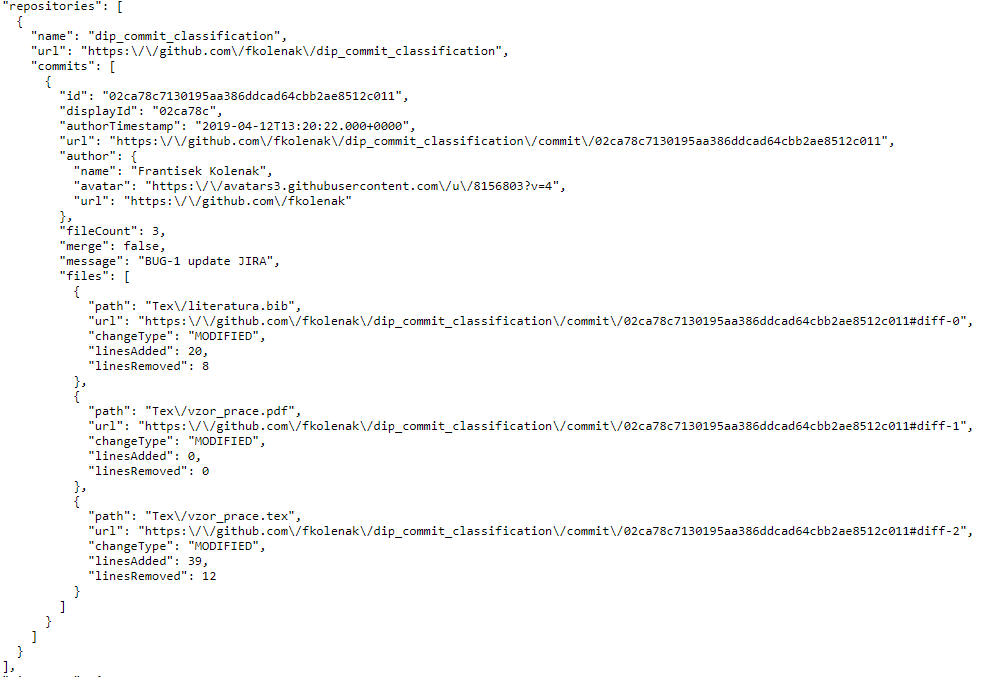
\includegraphics[width=1.0\textwidth]{Pic/JIRAresponse.png}
\end{center}
\label{pic:JIRAresponse}
\caption{Zkrácená odpověď na detail o commitech}
\end{figure}

\section{Github}




\section{Bugzilla}
Bugzilla\citep{bugzillabugtracking} je robustní a výkonný systém pro sledování defektů nebo systém pro sledování chyb. Má jednoduché funkce pro sledování defektů, které jsou zabudovány do integrovaných prostředí správy zdrojových kódů, jako jsou Github nebo jiné webové nebo lokálně nainstalované ekvivalenty. Bugzilla umožňuje správu pracovních postupů nebo kontrolu viditelnosti chyb (zabezpečení) nebo vlastní pole.

Bugzillu je možno upravovat podle libosti, neboť je open source. To znamená, že nejsou spojeny žádné náklady pro pořízení licence. Bugzilla má webové rozhraní a musí být nainstalována na vlastním serveru k tomu, aby ji bylo možno používat. To sebou nese výhody i nevýhody. Výhodou vlastního serveru je možnost uzavření serveru do vlastní sítě a tím pádem i zabezpečení. Nevýhodou jsou pak náklady na vlastní server a personál pro správu serveru.

Na obrázku Obrázek \ref{pic:bzLifecycle} je naznačen výchozí životní cyklus bugu. Tento cyklus se dá upravit podle potřeb organizace. Vlastnosti bugu se navíc dají upravit podle libosti.  Vzhledem k tomu že vlastnosti jsou si dost podobné, například oproti Jiře, je zbytečné všechny vyjmenovávat. Hlavními pořád zůstává popis, priorita a stav. Odlišností může být pole osobních značek, které jsou viditelné pouze pro autora značky. Toho se dá využít například pro snadné nalezení takto označeného bugu. Další zvláštností jsou \uv{flagy}. Ty mohou sloužit pro plánování, v tomto případě říkají, zda bude daný bug opraven nebo ne. 
\begin{figure}[!ht]
\begin{center}
	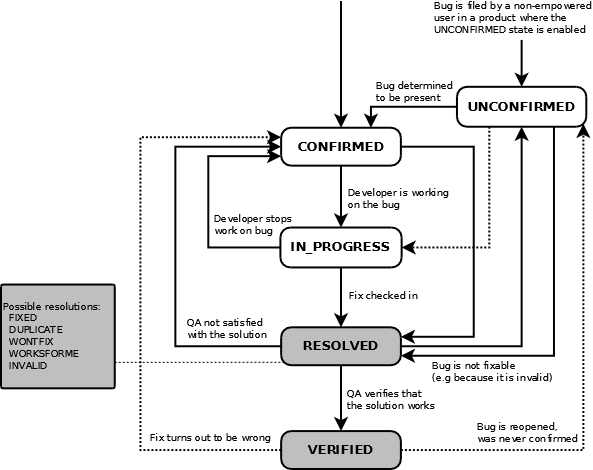
\includegraphics[width=1.0\textwidth]{Pic/bzLifecycle.png}
\end{center}
\label{pic:bzLifecycle}
\caption{Životní cyklus bugu. \citep{bugzillabugtracking}}
\end{figure}

Integrace s verzovacím systémem je velice jednoduchá, stačí připojit požadovaný systém k Bugzille. Po připojení se propojují commity pomocí jejich popisu. K propojení dojde pokud v commitu Bugzilla nalezne klíčová slova \uv{bug} nebo \uv{issue} a číslo daného bugu nebo problému. Příkladem pak může být následující commit: \uv{Tento commit opravuje \textit{issue 12, bug 18} a \textit{bug 92}.}. Od verze 5.0 nabízí Bugzilla i REST API, které je poté možno využít pro získání dat pro aplikace třetích stran. Pro starší verze Bugzilly je možné použít \textit{BzAPI}, které podporuje verzi 3.4 a vyšší, nevýhodou však je, že je to samostatný serverový software.

%NOTES https://wiki.mozilla.org/Bugzilla:REST_API https://bugzilla.readthedocs.io/en/latest/api/index.html
\section{Redmine}
Redmine je flexibilní webová aplikace pro projektový management. Je open source a jako ostatní konkurenti nabízí zajímavé funkce jako úpravu vlastností problémů, časových záznamů, projektů a uživatelů. Podporuje více projektů a ke každému nabízí řadu doplňkových funkcí: notifikace emailem, vlastní wiki stránky a nebo fórum pro každý projekt, sledování času, propojení s verzovacími systémy, vytvoření problému pomocí emailu, správa uživatelů a rolí uživatelů a mnoho dalšího.

Integrace s verzovacím systémem probíhá přímo pomocí Redmine. Je možno vytvořit nový repositář nebo spojit Redmine s již existujícím repositářem. Po načtení všeho potřebného je možno spojit commity s problémem nebo bugem. Redmine skenuje zprávy commitů pro reference problémů. Je možné také pomocí commit zprávy automaticky uzavřít náležící problém nebo bug. Po detekci funkce automatického uzavření, Redmine přiřadí náležitý status. Defaultní klíčová slova pro referenci na problém jsou: \textit{refs}, \textit{references}, \textit{IssueID}. Pro vyřešení problémů (v tomto případě bugů) jsou to klíčová slova: \textit{fixes} a \textit{closes}. Pro detekci musí být klíčové slovo odděleno od čísla reference mezerou a číslo reference musí začínat \#. V základu není nastaveno žádné klíčové slovo pro automatické uzavírání problémů, ale Redmine umožňuje nadefinování nového. Taktéž umožňuje nadefinování nových klíčových slov nebo úpravu stávajících, či dokonce nahrazení slova jen jako jednoduchou hvězdu (*). V případě poslední možnosti je jakékoliv nalezené ID spárováno s patřičným problémem.
Příkladem pak může být zpráva: \uv{This commit refs \#1, \#2 and fixes \#3}. Tato zpráva odkazuje na problém číslo 1 a 2 a opravuje problém číslo 3. Pro rozdělení jednotlivých referencí slouží znaky mezery čárky nebo \&.\cite{redminebugtracking}

Redmine poskytuje REST API pro těžení informací z repositáře. API podporuje základní CRUD operace (vytvoř, uprav a odstraň). V základu není API povoleno, proto je nutné ho povolit v nastavení projektu.

%TODO https://en.wikipedia.org/wiki/Comparison_of_issue-tracking_systems
%TODO Moznosti zapisovani bugu - github \href{https://en.wikipedia.org/wiki/Bug_tracking_system}{link4} 


%TODO pridani vyhody trackovani- snadna detekce duplikatu, klasifikace - prideleni odpovednym oddelenim, klasifikace - nejpravdepodobnejsi pricina, prioritizace \href{https://backlog.com/bug-tracking-guide/}{link5} 


%TODO zakladni klasifikace chyb



\chapter{Klasifikační metody}







 
% 
% PRO ANGLICKOU SAZBU JE NUTNÉ ZMĚNIT
% CITAČNÍ STYL!
%
\bibliographystyle{csplainnatkiv}
{\raggedright\small
\bibliography{literatura}
}

\end{document}
